%\documentclass[fleqn]{book}
\documentclass[11pt]{amsbook}

\usepackage[turkish]{babel}

%\usepackage{../HBSuerDemir}	% ------------------------
\usepackage{../Ceyhun}	% ------------------------
\usepackage{../amsTurkish}


\begin{document}
% ++++++++++++++++++++++++++++++++++++++
\hPage{084}
% ++++++++++++++++++++++++++++++++++++++
\subsection{Euler çizgeleri}
gibi sorular da euler çizgelerine yakın ilişkisi olan bulmacalrdır.

Şekil 2.5.4a daki çizimde 1 ve 2 düğümleri arasına bir ayrıt eklenmiş olsaydı, ortaya bir Euler çizgesi çıkacaktı. Öyleyse bu bulmaca, 1 ya da 2 düğümden başlanarak çözülebilir. Şekil 2.5.4b deki çözüme ilişkin, Şekil 2.5.5 deki çizgeyi düşünelim. Bu çizge bir Euler çizgesi değildir.

\begin{figure}[htb]
	\centering
	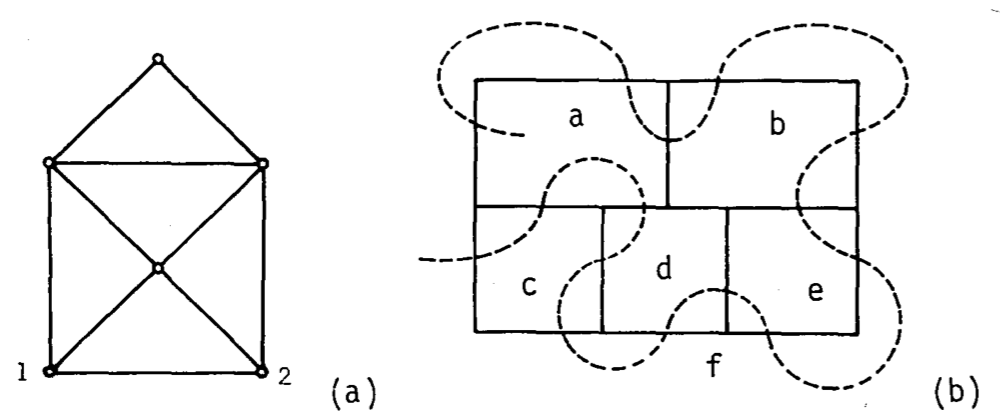
\includegraphics[width=0.45\textwidth]{images/ceyhun-084-fig01}
	\caption{Bulmacalar}
\end{figure}

Ancak bu çizgede kertesi teksayı olan dört düğüm olduğu için a, b, f ya da d den başlayarak , 16


\begin{figure}[htb]
	\centering
	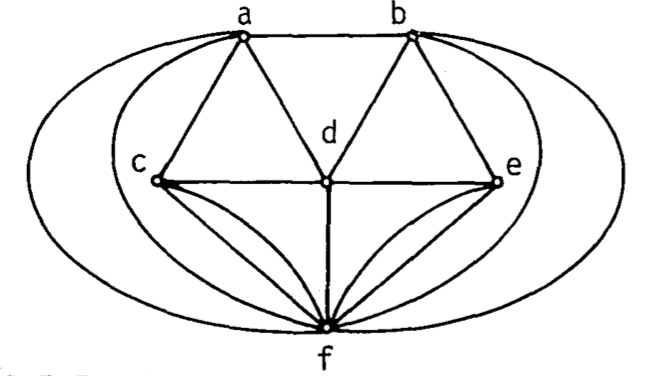
\includegraphics[width=0.45\textwidth]{images/ceyhun-084-fig02}
	\caption{Şekil 2.5.4b deki çizime ilişkin çizge}
\end{figure}



\end{document}